% chap3.tex (Definitions and Theorem)

\chapter{Provenance-Aware CPS (Prov-CPS)}

In this chapter, we explore the integration of provenance within the CPS ecosystem. We introduce Provenance-Aware CPS (Prov-CPS), a  provenance collection framework for CPS devices. We evaluate the effectiveness of our framework by developing a prototype system for proof of concept.

\section{Prov-CPS Design}\label{sec:design}

%In this section, we explain the integration of data provenance into the CPS ecosystem.
The first step to realizing the benefits that provenance offers for CPS is to develop a framework that collects provenance data from embedded systems in the CPS automatically and with minimal system overhead. Such a framework should be

\begin{enumerate}

\item \textbf{Complete:} A system must collect all provenance of causal dependencies between events. That is, provenance data collected must be complete in such a way that any datum can be backtracked to its source. % Completeness is defined by the application in which provenance data is used for. In our case, we utilize provenance graphs as input to our IDS system. 

\item \textbf{Abstract:} A system must be generic enough such that it can be reused across multiple CPS applications and domains. 

\end{enumerate}

Our approach leverages application-defined traces of data creation and transformation to achieve completeness, and uses a predefined provenance data model that is modular and generic to analyze those traces and convert them to provenance in a abstract manner.

% \textcolor{blue}{ We satisfy the conditions of completeness by developing a framework which is modular and generic in collecting trace data using a predefined abstract model as defined in \ref{prov_sensor}. Our model encapsulates the requirements for completeness while minimizing the amount of data that is stored.}

\section{Trace-based Provenance Data Model} \label{prov_sensor_model}

Embedded systems in a CPS application comprises of sensors and actuators operating on a continuous basis with data periodically created, transformed, and transmitted through device network interfaces. Properly representing these operations requires a data model that encompasses the intricate data flow within, between, and across devices. This model should be interoperable for varied application domains. 


Although provenance models are well-studied, no existing provenance model properly represents the dataflow of application logic for embedded systems in a CPS. To address this issue in Prov-CPS, we define a provenance-trace model that maps from the W3C's PROV-DM ontological representation to concepts relevant for a trace-based approach to provenance collection in a CPS. This mapping enables interoperability of Prov-CPS among heterogeneous systems and applications. 
Relationships between each component of provenance-trace model is depicted using relations as described in PROV-DM~\cite{prov_dm}. Table \ref{table_mapping_provenance} describes the mapping of terminology between the Prov-CPS trace-based provenance model and PROV-DM. 


\begin{table}[!tbh] \centering 
\caption{Concept mapping from trace-based provenance to PROV-DM.}
\label{table_mapping_provenance}
\resizebox{\textwidth}{!}{ \begin{tabular}{||c| c| c| c||} 
 \hline
 \textbf{Concept Description} &  \textbf{Provenance-trace model} &  \textbf{PROV-DM}  \\ [0.5ex] 
 \hline\hline
 Data to track with provenance & Data Object ($d)$ & Entity \\ 
 \hline
 Time at which provenance is produced & Timestamp ($t$) & Entity \\
 \hline
 Identity accountable for operations on data & Controller ($c$) & Agent \\
 \hline
 Identity components that creates, transforms, or transmits data & Producer ($p$) & Agent \\
 \hline
 Operations that create, transform, or transmit data & Action ($a$) & Activity \\ [1ex] 
 \hline
 \end{tabular}}
\end{table}

% There has been a couple of proposed data provenance models in the literature; however, there are no defined provenance model that properly represents information-flow of application-centric trace logic in a CPS device. To address this issue, we define a provenance-trace model on top of W3C Provenance ontology as a mapping of trace data to provenance ontological representation. This ensures interoperability between various heterogeneous systems that are contained in a CPS ecosystem. Our model satisfies the provenance characteristics as depicted in Section \ref{figure}. 

%%%Come back to this%%%%%%

%Figure \ref{prov_characteristics} represents an entity relationship diagram consisting of various components of the model and their interactions.

The Prov-CPS trace-based provenance model consists of five core components: data object, timestamp, controller, producer, and action. We define a data object as the information created, used, manipulated, or transmitted by a CPS. An action is work performed on a data object, such as creation, modification, or transmission, and a producer conducts the action on the data object.  A timestamp represents when an action occurred. A controller manages the actions of a producer; in the CPS setting at the embedded system level, the controller is the computing device.  A data object might be a result of another data object's modification by a producer, or an aggregated value including multiple data objects, where the aggregated value is contained in a transformed data object with a provenance relationship to the data objects included in its aggregation. The software that calculates the aggregate is the producer. 

Consider the periodic temperature readings taken by a thermostat as a simple example mapping between an application domain and the trace-based provenance model. In this example, the thermostat itself is the controller, the data object is a temperature reading, the producer is a temperature sensor, the action is reading of the sensor, and the timestamp is the thermostat's notion of time when the reading was taken.

The key to effective collection of provenance is the definition of a general trace event format that is applicable to multiple applications and varied operations on data. We define a trace event record as a tuple 
 \[ event_{trace} = (t, d, a, c, p ) \] 
 where $t$ is a timestamp, $d$ is a data object, $a$ is an action, $c$ is a controller's identifier, and $p$ is a producer's identifier.

For every trace event, Prov-CPS establishes the following fixed relationships between the provenance model components:
\begin{enumerate}
 \item $c$ \textit{used} $p$
 \item $(t,d)$ \textit{wasGeneratedBy} $a$
 \item $p$ \textit{wasAssociatedWith} $a$
 \item $(t,d)_{p}$ \textit{wasAssociatedWith} $(t,d)$
\end{enumerate}
where $(t,d)_{p}$ is the most recent $(t,d)$ generated by an action associated with the producer $p$. This last relationship establishes a temporal relationship between data objects generated by the same producer.

% To denote relations, each node forms an edge with a specified node as follows:
 
% \begin{itemize}
% 
% \item $c$ forms  \textit{actedOnbehalfOf} with $p$
% \item  $S$ forms a \textit{wasGeneratedBy} edge with activity $a$.
% \item  $a$ forms a \textit{wasGeneratedBy} edge with data object $d$.
% \end{itemize}
% 
% where $t$ is a timestamp, $d$ denotes a data object, $a$  denotes an activity, and $c$,  $p$ denotes controller and producer agents respectively 

% A sensor device might possess the ability to generate multiple trace data, $td$. For instance, a sensor device might be able to generate sensor data consisting of temperature and humidity values. A combination of trace data at a particular point is considered an event. We define an event  for sensor $s_1$ at time $t$ as $e= \{td_1, ...td_n\} $ where $td_1$ represents the first data generated by $s_1$  and $td_n$ is the last trace generated which occurs at time $t$. Trace data is mapped to a provenance ontology types in which an  Agent represents device and sensor identifier, an activity represents actions performed on the device (e.g., read, update, create, delete) , an entity represents a trace event (e.g., temperature reading). Each trace data is represented as a tuple $(t, e, a, s_1, r_1)$ where $t$ is a timestamp, $e$ denotes an event, $a$ denotes an activity, $s_1$ denotes a sensor identifier and $r_1$ denotes a device identifier. Table \ref{prov_sensor} displays a detailed list of concepts in IoT device mapped to a provenance ontology.

\begin{figure}[h!]
\begin{center}

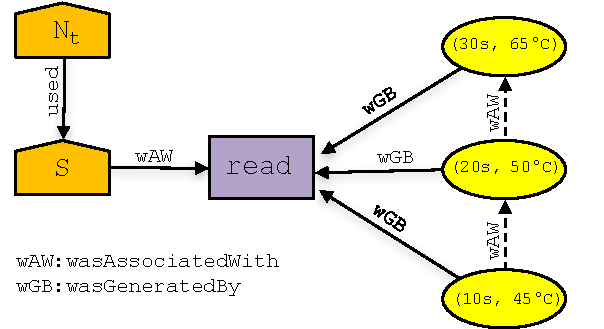
\includegraphics[width=0.6\textwidth]{prov_sensor_v3.pdf}
\end{center}
\caption{Provenance graph generated from a thermostat device.}
\label{prov_sensor}
\end{figure}

\subsubsection{Example: Thermostat}

We demonstrate the Prov-CPS data model with an example of thermostat device ($N_t$) containing a sensor ($S$) that generates temperature readings at a time interval of 10 seconds. Temperature readings of the first 3 consecutive data objects are 45 $\degree$C, 50 $\degree$C, and 65 $\degree$C respectively. Trace events generated for these first three data objects are
\[event_{trace1} = (10 s, 45 ^{\circ}C, read, N_t, S)\]  
\[event_{trace2} = (20 s, 50 ^{\circ}C, read, N_t, S)\]  
\[event_{trace3} = (30 s, 65 ^{\circ}C, read, N_t, S)\]
Relations between components of the trace event are formed as described earlier. $N_t$ forms a \textit{used} edge with $S$, which itself forms a \textit{wasAssociatedWith} edge with the $read$ action. Each temperature reading's timestamp and data object are grouped as a pair ($t, d$) and form a \textit{wasGeneratedBy} edge with the $read$ action and a \textit{wasAssociatedWith} edge with the previous pair associated with $S$ through the $read$ action that generated it. Figure~\ref{prov_sensor} depicts the provenance graph for this thermostat example.



% in which a temperature sensor $s_1$, is connected to device $r_1$. Data object $d$ consists of a set of temperature and humidity values ($i.e., d = \{temperature, humidity\}$). Therefore the tuple representation of trace data for sensor $s_1$ at time $t_1$ is $(t_1, \{temperature, humidity\}, a,  s_1, r_1)$. Since $s_1$ is contained in device $r_1$, $r_1$ forms an edge with $s_1$ with the \textit{actedonbehalfof} relation. (e.g $r_1$ used $s_1$) and $s_1$ forms a \textit{wasGeneratedBy} edge with $a$, activity $a$ forms an \textit{wasusedBy} edge with event $e$. Algorithm \ref{prov_to_trace} further illustrates how a provenance graph can be generated using the provenance-sensor model.





%Sensor data contains observational information such as temperature, and location details which can be transformed to standardized data interchange formats (RDF, XML, JSON). Sensor data are time series data which can be traced over time. Trace data containing sensor readings are important but do not depict dependency relationships when used alone. We transform trace data to provenance to represent causality and dependency relationships between entities in an IoT system. Provenance can be represented as a directed acyclic graph and the edge between two entities is considered a relation. Relations between data objects follows provenance ontology which depicts transformation between entities. We integrate PROV-O and sensor data for better representation of dependency relationships between trace data generated.
%
%\par A single sensor might posses the ability to collect multiple trace data, $td$. For example, a sensor might be able to collect sensor readings of temperature, location, humidity. A combination of trace data at a particular point in time is considered an event. We define an event  for sensor $s_1$ at time $t$ as $e= \{td_1, ...td_n\} $ where $td_1$ is the first trace data collected by $s_1$  and $td_n$ is the last which occurs at time $t$.
%
%\par Adopting provenance ontology to IoT, we represent device information as agents (prov:agents), the operation performed on sensor readings (read, create, update) as a provenance activity (prov:activity), and events as entities (prov:entity). A sensor trace is defined as a tuple  $ (t, e, a, s_1, r_1)$ where $t$ represents a timestamp, $e$ an event, $a$ an operation, $s_1$ sensor information and $r_1$ device information.  

%\begin{algorithm}  
%
%\caption{Provenance-trace Model.}
%\label{prov_to_trace}
%\begin{algorithmic}[1]
%\Procedure{trace2Prov}{$ts$}
%\State \textbf{INPUT: } $ts \gets$ set of trace trace event
%%\State $E_G \gets \{\}$
%%\For{$p_i = (V_i, E_i) \in P, 0 \leq i \leq n$}
%\State $e_{list} \gets \{\}$
%\
%\State $pd \gets pd.createProvDocument()$
%
%\For{  $(t, d, e, c, p \in ts$}
%
%\If{  $c \not\in pd$}
%\State  $ag_c \gets pd.createAgent(c)$
%\EndIf
%
%\If{  $ p \not\in pd$ }
%\State $ag_p \gets pd.createAgent(p)$ 
%\EndIf
%
%\State $dt = \{d, t\}$ 
%
%\State $entity \gets pd.createEntity(dt)$  
%
%\State $e_{list} \gets e_{list} \cup  entity$
%
%\State $activity \gets pd.createActivity(a)$ 
%
%
%\If{$ used \not\in pd$}
% \State  $ pd.used( c, p)$ 
% \EndIf
%
%\State  $pd.wasAssociatedWith(a, c)$
%
% \State $ pd.wasGeneratedBy(a, dt)$ 
% 
% \If{ $counter > 0$}
% \State $ pd.wasAssociatedWith( e_{list}[counter - 1],  entity)$
% \EndIf
% 
%\State $counter = counter + 1$
% 
% \EndFor
%%\EndFor
%\State \textbf{return} $pd$
%\EndProcedure
%
%\end{algorithmic}
%\end{algorithm}

%%%% FIXME: This is wrong. Fix it, or remove it.
%\begin{algorithm}  
%
%\caption{Provenance-trace Model.}
%\label{prov_to_trace}
%\begin{algorithmic}[1]
%\Procedure{Provtrace}{$ts$}
%\State \textbf{INPUT: } $ts \gets$ set of trace trace event
%%\State $E_G \gets \{\}$
%%\For{$p_i = (V_i, E_i) \in P, 0 \leq i \leq n$}
%\State $i = 0$
%\State $e_{list} \gets \{\}$
%\
%\State $pd \gets createProvDocument()$
%
%\For{  $(t, d, a, c, p) \in ts$}
%
%
%\State  $ag_c \gets pd.createAgent(c)$
%\State $ag_p \gets pd.createAgent(p)$ 
%
%\State $entity \gets pd.createEntity(d,t)$  
%\State $e_{list} \gets e_{list} \cup  entity$
%\State $ pd.wasAssociatedWith( e_{list}[i - 1],  e_{list}[i])$ 
%
%\State $activity \gets pd.createActivity(a)$ 
%\State  $ pd.used( ag_c, ag_p)$ 
%\State $pd.wasAssociatedWith(activity, ag_c)$
%\State $ pd.wasGeneratedBy(a, e_{list}[i])$ 
%
%
%\State $i = i+1$
% 
% \EndFor
%%\EndFor
%\State \textbf{return} $pd$
%\EndProcedure
%
%\end{algorithmic}
%\end{algorithm}


\section{Prov-CPS Architecture}
Prov-CPS uses a modular approach that decouples the act of tracing events from that of linking them to form provenance. In this section we describe the architectural design of this approach, and defer implementation details to Section~\ref{system_implementation}.  Figure \ref{framework_design} illustrates the overall system design consisting of four primary components:

%An example of system events are events generated from application source code such as variable, function values or OS system call. Data trace is collected at the tracer component. The resulting output is converted into an appropriate provenance graph representation at the Trace Mapper component using our provenance-trace model as discussed in Section \ref{prov_sensor_model}. The resulting provenance graph generated is stored in a graph database (e.g., Neo4j) for further processing. The generated provenance graph can be used as input to a provenance application of choice. We give a detailed description of components of our framework below:
 
 \textbf{Tracer} is a program located on the CPS device that is responsible for generating trace data from application-level data events. 
  
 \textbf{Trace mapper} converts trace data into a provenance graph representation using the ProvCPS data model in which trace events are mapped to provenance and relationships between them are established.
 
 \textbf{Graph database} is used to store provenance data for further processing. A graph database such as Neo4j is an ideal choice because it allows for easy graph traversal and querying analytics.
 
 \textbf{Provenance application} uses provenance data for specific tasks such as anomaly detection or digital forensics. %For our implementation, we chose to utilize provenance graphs for intrusion detection since we can detect event states changes through causality and dependencies derived from Prov-CPS.
 
 \begin{figure}[h!]
\begin{center}
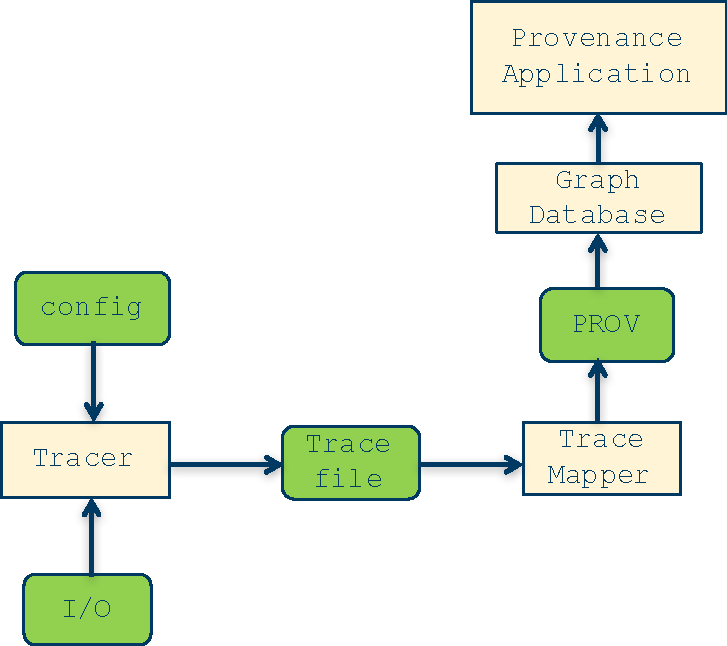
\includegraphics[width=0.6\textwidth]{sys_arc_3_6.pdf}
\end{center}
\caption{Prov-CPS Conceptual System Design.}
\label{framework_design}
\end{figure}

\section{System Implementation} \label{system_implementation}

Figure~\ref{figure} depicts our implementation of the architectural components of Prov-CPS. For the tracer component we use \textbf{barectf}~\cite{barectf}, which is a program for tracing applications written in the C programming language specifically meant for execution on bare-metal devices (devices without an operating system). We chose this program is lightweight, portable, and allows for implementation on memory constrained embedded systems.
%
%since most embedded systems consist of no operating system
%
Barectf generates trace functions that can be called from an application's source code. The event field traced corresponds to values of variables or functions in the application source code that are specified as parameters of the trace function. 
%
%
%Figure~\ref{figure} illustrates source code instrumentation of trace functions in a simplistic temperature and humidity IoT application implemented on a raspberry Pi system.  Trace functions are embedded into the temperature application using functions generated from barectf. Trace function parameter represents event fields of sensor data to be traced. Code fragments highlighted in grey represents trace functions invocation.
%
%%%%Insert source code here... %%%%
%
Event field specification is done by a using a configuration file written in the \textbf{yaml} language from which the trace functions are automatically generated by barectf. At execution time, the trace functions generate trace output to a stream object in \textbf{common trace format} (CTF)~\cite{ctf} packets. CTF is a fast binary trace format for representing trace data.

We implemented a trace mapper on top of the babeltrace~\cite{babeltrace} python bindings for programmatically manipulating CTF streams. With babeltrace, we are able to access trace packets contained in a CTF packet stream and convert them to a provenance graph representation. To generate provenance graphs, we utilize the \textbf{PROV} python library for creating W3C compliant provenance ontology documents. The provenance graph generated is serialized into an intermediate file in JSON format that can be stored in Neo4j for efficient query and graph processing.

The provenance application we use to evaluate Prov-CPS in this work is a graph-based anomaly detection algorithm for use as a CPS intrusion detection system, which we describe in chapter~\ref{sec:prov_anomaly}.

 \begin{figure}[h!]
\begin{center}
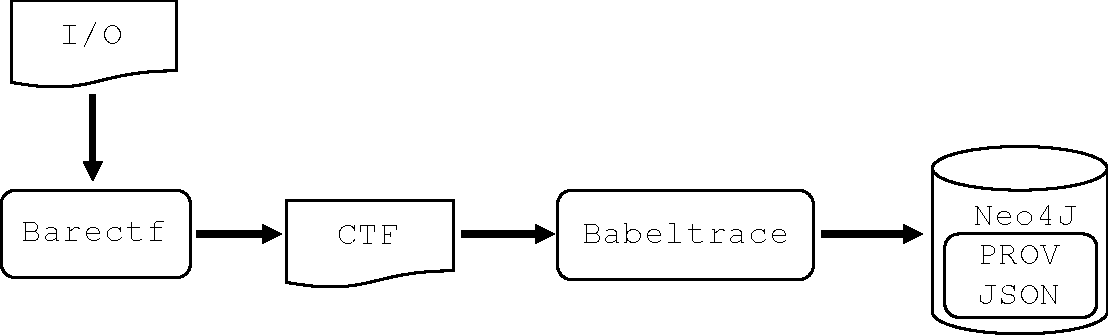
\includegraphics[width=0.6\textwidth]{system_implementation_v4.pdf}
\end{center}
\caption{Prov-CPS System Implementation.}
\label{figure}
\end{figure}

 \subsection{Complexity analysis}
%This section analyzes time and space complexity of the various components contained in Prov-CPS. 

\textbf{Tracer} appends trace data to a list of events. This takes $O(1)$ time and $O(n)$ space. \textbf{Trace mapper} iterates through all of the events and maps them to PROV-O using Provenance-trace model. This takes $O(n)$ time and $O(n)$ space.

\section{Summary}
This chapter introduces PROV-CPS, a provenance collection framework for CPS devices. Components of PROV-CPS such as tracer and trace mapper are discussed with system implementation details. The next chapter discusses storage optimization techniques for provenance data generated in PROV-CPS.







 